\documentclass[a4paper, 9pt,twocolumn,dvipdfmx]{jsarticle}

%\usepackage[a4paper,top=10truemm,bottom=10truemm,left=1truemm,right=1truemm]{geometry}
\usepackage{amsmath}
\usepackage{amsfonts}
\usepackage{eshouroku}
\usepackage[dvipdfmx]{graphicx}
\usepackage{amsmath}
\usepackage{url}
\usepackage{here}
\usepackage{booktabs}
\usepackage{remreset}
\usepackage{pdfpages}
\usepackage{comment}
\usepackage{subfigure}
\usepackage{amsmath}
\usepackage{titlesec}
\pagestyle{empty}
\setlength{\columnsep}{2zw}
\newcommand{\ctext}[1]{\raise0.2ex\hbox{\textcircled{\scriptsize{#1}}}}

\titleformat*{\section}{\normalsize\bfseries}
\titleformat*{\subsection}{\small\bfseries}
\titleformat*{\subsubsection}{\small\bfseries}
\renewcommand{\baselinestretch}{0.945}

\renewcommand{\subfigtopskip}{1pt}	% 図の上の隙間。上図の副題と下図の間。
\renewcommand{\subfigbottomskip}{0pt} % 図の下の隙間。副題と本題の間。
\renewcommand{\subfigcapskip}{-6pt}	% 図と副題の間
\renewcommand{\subcapsize}{\scriptsize} % 副題の文字の大きさ

\makeatletter
	\renewcommand{\theequation}{% 式番号の付け方
	\thesection\arabic{equation}}
	\@addtoreset{equation}{section}

	\renewcommand{\thefigure}{% 図番号の付け方
	\thesection\arabic{figure}}
	\@addtoreset{figure}{section}

	\renewcommand{\thetable}{% 表番号の付け方
	\thesection\arabic{table}}
	\@addtoreset{table}{section}
\makeatother
%\numberwithin{equation}{section}
%\numberwithin{table}{section}
%\numberwithin{figure}{section}


% 数式(演算子など)のスペースを詰める
% =,→ 間の余白
\thickmuskip=1.0\thickmuskip
% +,- 間の余白
\medmuskip=0.8\medmuskip
% … などの装飾記号の余白
\thinmuskip=0.8\thinmuskip
% 行列を詰める
\arraycolsep=0.3\arraycolsep
% 数式の上下のスペースの変更
\AtBeginDocument{
  \abovedisplayskip     =0.5\abovedisplayskip
  \abovedisplayshortskip=0.5\abovedisplayshortskip
  \belowdisplayskip     =0.5\belowdisplayskip
  \belowdisplayshortskip=0.5\belowdisplayshortskip}


%\boldmainfalse% 主文を普通文字にするモード(抄録印刷時はこちら)
\graphicspath{{./figs}}

\begin{document}

\twocolumn[
 \講演番号{B-11}% 必要ない場合には書かない
 \日本語タイトル{\huge}{神経免疫相互作用に着想を得た\\マルチエージェントシステム型ニューラルネットワークの提案}
 \英語タイトル{\large}{Proposal of Neural Network composed of Multi-Agent System Inspired by Neuroimmune Interaction}
 \筆者一名{5335}{柚木開登}

 \指導教員一名{山本哲也}
 %\指導教員二名{東京花子}{京都紀夫}
 %\指導教員なし
]
%\addcontentsline{toc}{section}{\refname}% 追加

\graphicspath{{./figs/}} % 図が特定のフォルダにある場合には設定

\section{本研究の意義・目的}
\begin{comment}
本来的に大規模な計算資源を必要とするニューラルネットワークが
今日, あらゆる産業へ導入されるに至ったのは, クラウドコンピューティングの貢献がある.
一方で, 同市場拡大に伴って
プラットフォーマによる市場寡占, データセンターでの電力消費, データプライバシーの課題が表面化した.
こうしたクラウドの課題克服に向けて, 
データを集約せずにネットワークの端点(エッジ)で処理するエッジコンピューティングが注目
されている.
\end{comment}
エッジコンピューティングパラダイムにおける機械学習手法として
連合学習(Federareted Lerning)が提案されている\cite{DFL}.
連合学習では, 
ローカルデータを保有する複数のノードが内部で学習を行い, 
学習パラメータの差分情報のみを通信し, 
平均化することで大規模な学習済みモデルを構築する.
これにより, 従来, データセンターに集約されていた
プライバシーを含んだ学習データは各ノード内に完全に保護される.
GDPRをはじめとする世界的な個人情報保護の動きの高まりから, 
将来的に連合学習は情報社会において重要な位置を占めることが予想される.

一方, 連合学習では
計算資源に乏しいエッジ環境内で学習させるため, 
大規模なモデルを投入することが難しいという課題がある.
この課題解決には, モデルの軽量化と
分散処理による環境内計算資源の利用の最大化という両方面からのアプローチが重要になる.
この2種の手法を満たすモデルは
連合学習の実用化に貢献するものと期待できるが, 
両者を兼ね備えたモデルに関する研究は著者の知る限り存在しない. 

そこで本研究では,  
所望の計算サイズに分散可能で, 
自律的にパラメータ削減を行いモデルを軽量化するニューラルネットワークを提案する(\wfig{ThisModel}).
\vspace{-1.5zh}
\begin{figure}[H]
  \centering
  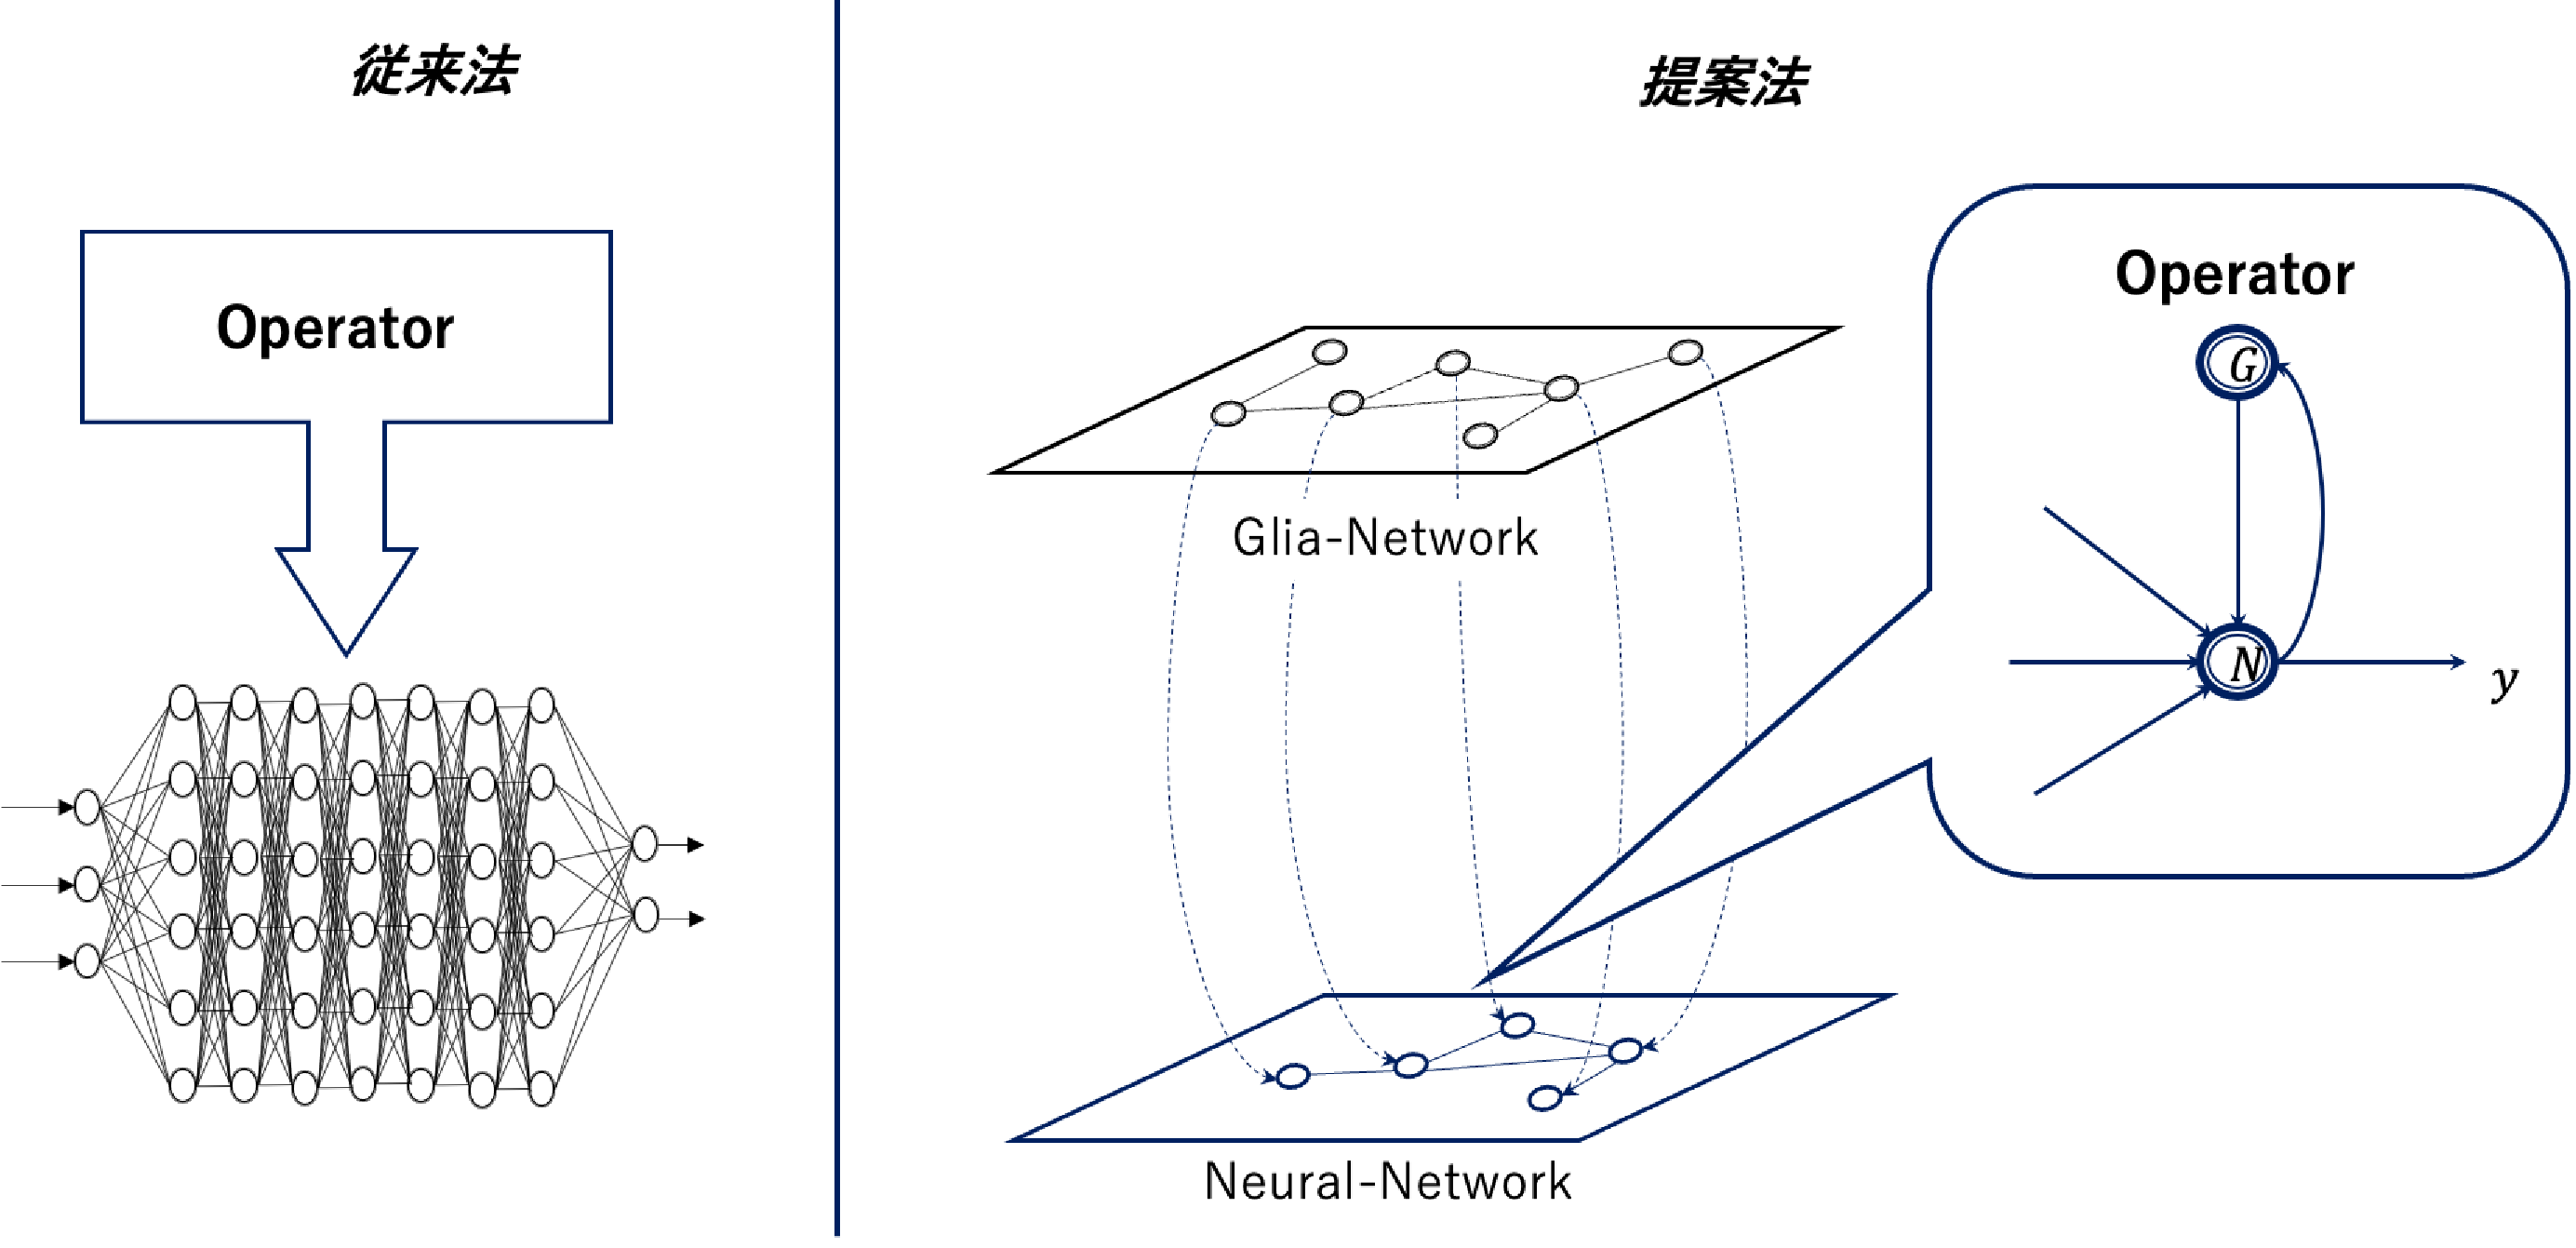
\includegraphics[width=7cm]{ThisModel.pdf}
  \caption{従来法と提案法の比較}
  \label{fig:ThisModel}
\end{figure}
\vspace{-3zh}
\section{提案モデル}
\subsection{複数のエージェントによるニューラルネットワーク}
パラメータ削減にあたって, 脳内免疫細胞であるmicrogliaによるシナプスの刈り込み作用に着目し, 
これに関与する各パラメータをエージェント(自律行動主体)としてモデル化した上で, これらの相互作用に拠って
システム全体を構成している. 
以下, 投入するエージェントについて説明する.
\vspace{2mm}
  \subsubsection*{●Neuro-Agent;\,\,}
  神経細胞をモデル化したエージェントであり, 情報の受容, 処理, 
  転送などを担当する.
  それぞれのNeuro-Agentは, 情報を受け取るための複数の入力$x_i$ $\;(i= 1, 2, 3, \cdots m)$と, 
  内部変数$b$を持ち, 
  これを処理して別のNeuro-Agentに情報を送信するための出力$y$を生成する.
  この時の内部処理は\weq{Neuro-Agent}に示す通り, 
  標準的な人工ニューロンと同等に活性化関数$\phi$を用いた変換である.
  \begin{align}
    y=\phi(\sum_{i=1}^m x_i+b)
    \label{eq:Neuro-Agent}
  \end{align}
  \subsubsection*{●Synapse-Agent;\,\,}
  神経回路における接触構造であるシナプスをモデル化したエージェントであり, 
  Neuro-Agent間の情報の伝達を担当する.
  それぞれのSynapse-Agentは, 入力$u$を受け取り, それを変換した値$v$を出力する(\weq{Synapse-Agent}). 
  この出力は別のNeuro-Agentの入力$x_i, i\in\mathbb{N}^+$として使用される.
  \begin{align}
    v=weight\cdot u
 \label{eq:Synapse-Agent}   
  \end{align}
  ここで, 式中の$weight$は, そのSynapse-Agentの重みを示し, 
  これとNeuro-Agentの内部変数$b$を誤差逆伝播法を用いて更新することで, ニューラルネットワークが学習される.
  \vspace{2mm}
  \subsubsection*{●Glia-Agent;\,\,}
  神経細胞の補助細胞であるグリア細胞(Glia-Cell)の機能を模倣したエージェント.
  Glia-Agentは, Neuro-AgentとSynapse-Agentによって構成されるニューラルネットワークに対して,
  シナプスの刈り込みを行い, パラメータ削減による学習の効率化・高速化を試みる. 
  \vspace{2mm}
\subsection{神経免疫相互作用に基づく相互調節モデル}
神経系と免疫系は独立したシステムではなく
神経免疫相互作用(Neuroimmune Interaction)と呼ばれる相互調節機構を持つ.
殊に生体の脳機能発達においては, 神経細胞からのシグナル伝達に拠って
グリア細胞(microglia)が神経回路の刈り込みを行うことが確認されている.
本モデルではこれをNeuro-AgentとGlia-Agent間の相互作用として組み込んだ.
\vspace{-5mm}
\begin{figure}[H]
  \centering
  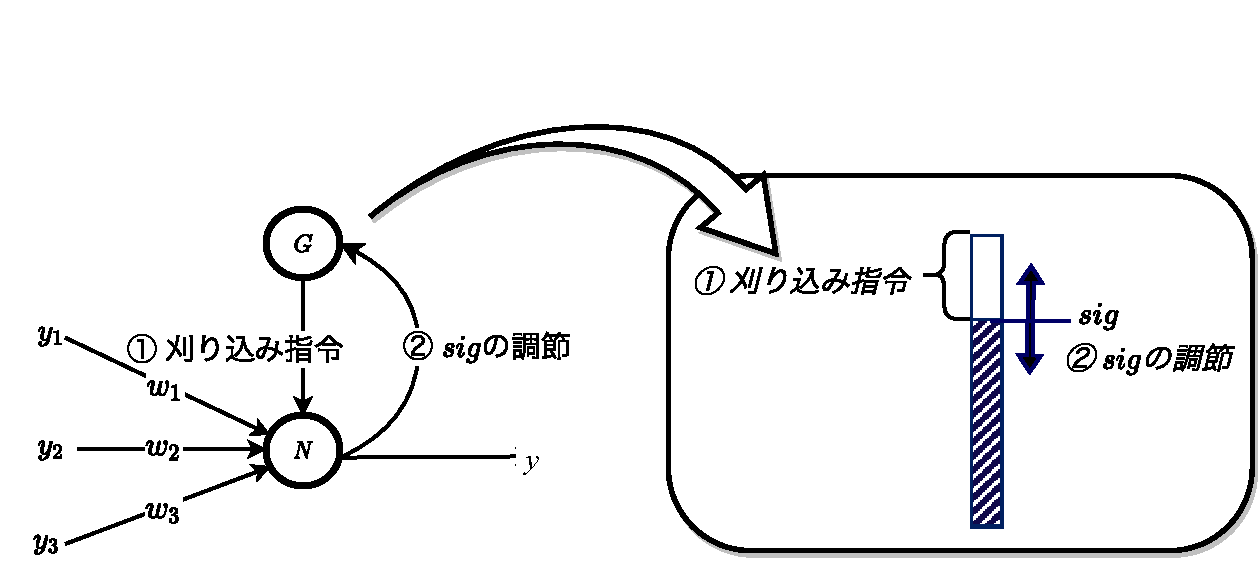
\includegraphics[width=9cm]{NewDeal.pdf}  
  \caption{Neuro-Glia相互調節機構}
  \label{fig:NeuroGlia}
\end{figure}
\vspace{-5mm}
\wfig{NeuroGlia}に示すようにGlia-AgentとNeuro-Agentは1:1で接続され, 
 適宜Glia-Agentの内部変数$sig$を更新していくことで刈り込みの制御を行う.
 \vspace{1mm}
\subsubsection*{Glia-AgentからNeuro-Agentへの作用\,\,:\,\,刈り込み命令の発出}
シナプスの刈り込み命令はGlia-Agentの内部変数$sig$
を閾値に用いて確率的に実行される.
Neuro-Agentは刈り込み命令を受け取ると, 自身に接続された最も重みが0に近いSynapse-Agentを
削除する.
また, 刈り込み指令を発出したGlia-Agentは
$sig=1.0$に更新し, グリアネットワークへの伝播を行う.
詳しくは2.3節で述べるが, これに拠って時空間的に集中した過度な刈り込みが抑制される.
\subsubsection*{Neuro-AgentからGlia-Agentへの作用\,\,:\,\,$sig$の更新}
Neuro-Agentはまず, $miniBatchSize$の間に
隣接するNeuro-Agentの出力値と比較し, 自分が外れ値であった回数を変数$cnt$にカウントする.
次に, $cnt$を用いて自身の活動頻度$freq$を計算する.
\begin{align}
  freq=\displaystyle\frac{cnt}{miniBatchSize}
\end{align}
最後に$freq$を用いて, Glia-Agentの内部変数$sig$を更新する.
$sig$の更新式は\weq{sig}に示す通りである. 
ただし, わかりやすさのため式中でGlia-Agentのプロパティには$G$, 及び
Neuro-Agentのプロパティには$N$の添字を付してある.
\begin{align}
  sig_G\leftarrow sig_G-&\alpha\left[\cfrac{2}{1-\beta\exp(freq_N-0.01)}-1\right]
  \label{eq:sig}
\end{align}
\weq{sig}は, Neuro-Agentの活動頻度$freq$が高いほど刈り込みを抑制し, 逆に$freq$が小さいほど
刈り込みがされやすくなるように$sig$を更新する.
\subsection{グリアネットワークによる過度な刈り込みの抑制}
ASDや統合失調症などの神経免疫疾患の報告からシナプスの刈り込みが脳の高次機能維持・発現の要因である可能性が示唆されている.
これは同時に, グリア細胞による過度な刈り込みを抑制するシステムの存在が仮定するものであり医学的解明が急がれる.
我々はこのシステムの在処として, グリア細胞同士のネットワークであるグリアアセンブリ(Glia-Assembly)
であると仮定し, あるGlia-Agentが刈り込み指令を下した際に, 
そのエージェントの$sig$を他のGlia-Agentに伝達し影響させ過度な刈り込みを抑制させる
Glia-Agent同士のネットワーク; グリアネットワークを模倣・実装した.
グリアネットワーク上において$sig$は伝播距離(ホップ数)に応じて減衰定数$A$だけ減衰していく.
なお, 複数の距離が与えられた場合, 最も近い$Glia-Agent$の影響を優先する.
例えば, \wfig{GliaNetworks}の$g_2$の場合, 
$g_0\rightarrow g_1\rightarrow g_2$と$g_0\rightarrow g_2$の経路では後者の経路のみを考えることになる.
\vspace{-5mm}
\begin{figure}[H]
  \centering
  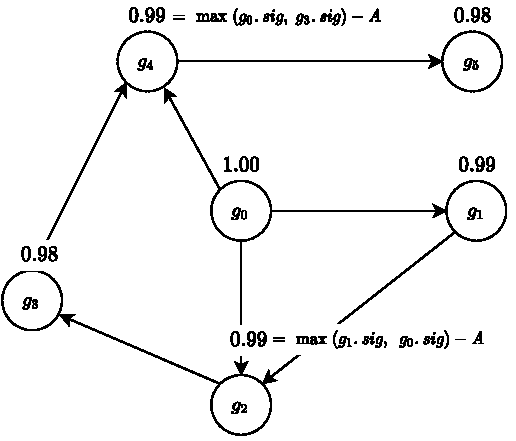
\includegraphics[width=8cm]{GliaNetworks.pdf}
  \caption{グリアネットワークでの$sig$の伝播のあり方}
  \label{fig:GliaNetworks}
\end{figure}
\vspace{-4mm}
\section{計算機実験}
計算機実験として$6\rightarrow 8\rightarrow 8\rightarrow 8\rightarrow 1$の
5層全結合ニューラルネットワークを用意し, 
6bitの入力の上位3bitのいずれかに1が入っているかどうか
の判別のタスクを行った.
その他のパラメータは以下に示す通りである(\wtab{param}).
\vspace{-0.5cm}
\begin{table}[H]
  \caption{パラメータ一覧}
  \label{tab:param}
  \centering
  \scalebox{0.9}{
   \begin{tabular}{ll}
    \toprule
      パラメータ&値\\\midrule\midrule
      学習率$\eta$&$0.5$\\
      エポック数$Epocs$&$100$\\
      ミニバッチサイズ$miniBatchSize$&$100$\\
      初期ニューロン数$Neurons$&$31$\\
      初期グリア数$Glias$&$31$\\
      初期抑制信号値$sig$&0.5\\
      初期シナプス数$Mill$&$182$\\
      減衰率$A$&0.01\\
      入力サイズ$Inputs$&$6$\\
      出力サイズ$Outputs$&$1$\\
      チューニングパラメータ$\alpha$&0.01\\
      チューニングパラメータ$\beta$&$6\ln(3)$\\
    \bottomrule
   \end{tabular}
  }
 \end{table}
計算機実験の結果得られた学習曲線及びシナプス数の変化及び, 刈り込み後のネットワークを\wfig{LearningCurve}, 
\wfig{SynapseNum}及び\wfig{Graph}に示す.
\begin{figure}[H]
  \centering
  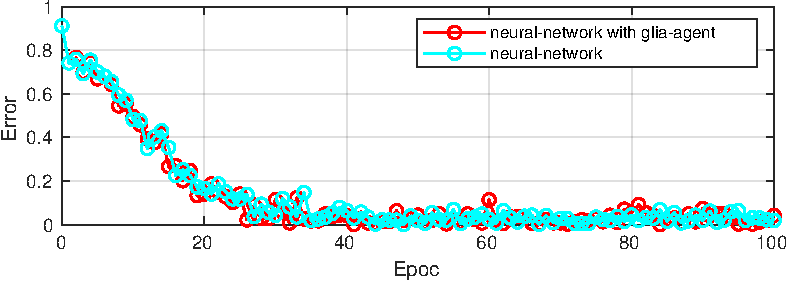
\includegraphics[width=8cm]{LearningCurve-crop.pdf} 
  \caption{学習曲線}
  \label{fig:LearningCurve}
\end{figure}
\vspace{-2zh}
\begin{figure}[H]
  \centering
  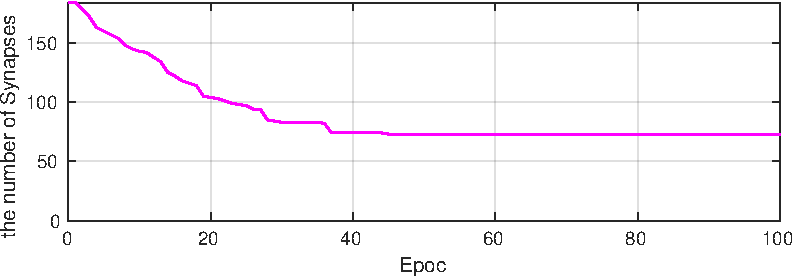
\includegraphics[width=8cm]{SynapseNum-crop.pdf} 
  \caption{シナプス量の変化}
  \label{fig:SynapseNum}
\end{figure}
\vspace{-2zh}
\begin{figure}[H]
  \centering
  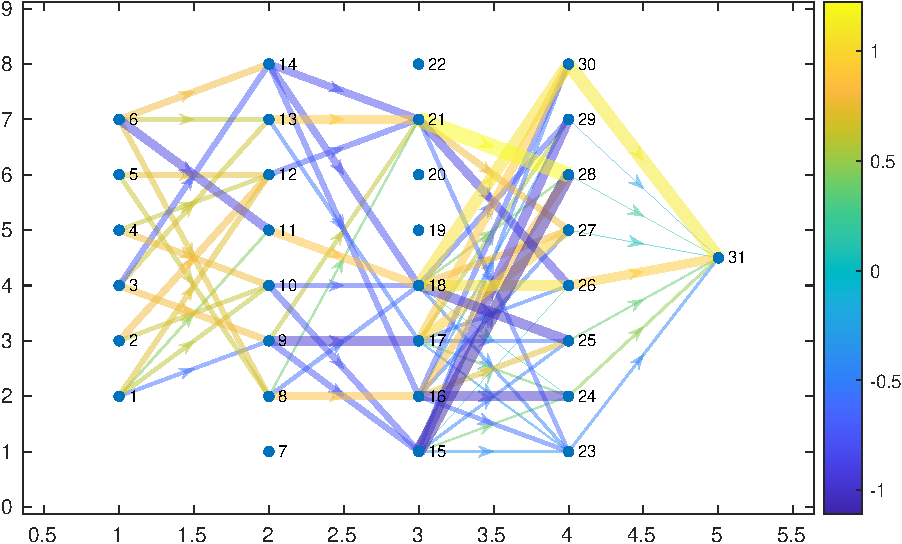
\includegraphics[width=7cm]{Graph-crop.pdf} 
  \caption{刈り込み後のネットワーク}
  \label{fig:Graph}
\end{figure}
Glia-Agent及びグリアネットワークによる刈り込みを実行した結果, 最終的なシナプス数は$182$から$72$に推移した. 
また, この時の学習曲線は刈り込みを行わない場合と比較してほとんど同一の曲線を描き, 
精度の悪化が認められない.
従って, 60%のシナプスの削減が精度を維持したまま行われたと評価できる.
\section{結論}
神経免疫相互作用に着想を得て全体の管理者のいない
ニューラルネットワークの学習パラメータの削減を実装し, 
学習精度を落とさない適切な刈り込みを行うことができた.
興味深いのはシナプス数の減少曲線が, 生体の脳で行われる
オーバーシュート型シナプス形成と同様に, 
指数関数的な減少を見せていることである. 
曲線のあり方が今後どのように影響するのか, 
あるいはグリアネットワークの構造が
曲線にどのように影響するのかなど, 
各パラメータの在り方については今後の課題とする.
 \begin{thebibliography}{99}
  \bibitem{DFL} 	
  Roy, Abhijit Guha, et al. "Braintorrent: A peer-to-peer environment for decentralized federated learning." arXiv preprint arXiv:1905.06731 (2019).
  \bibitem{ADIPS}
  藤田茂, et al. "分散処理システムのエージェント指向アーキテクチャ." 情報処理学会論文誌 37.5 (1996): 840-852.
\end{thebibliography}
 \end{document}
